\documentclass[]{article}

\usepackage{lmodern}
\usepackage{amssymb,amsmath}
\usepackage{ifxetex,ifluatex}
\usepackage{fixltx2e} % provides \textsubscript
\usepackage[a4paper, total={6in, 10in}]{geometry}
\ifnum 0\ifxetex 1\fi\ifluatex 1\fi=0 % if pdftex
  \usepackage[T1]{fontenc}
  \usepackage[utf8]{inputenc}
  \usepackage[english,russian]{babel}
\else % if luatex or xelatex
  \ifxetex
    \usepackage{mathspec}
  \else
    \usepackage{fontspec}
  \fi
  \defaultfontfeatures{Ligatures=TeX,Scale=MatchLowercase}
\fi
% use upquote if available, for straight quotes in verbatim environments
\IfFileExists{upquote.sty}{\usepackage{upquote}}{}
% use microtype if available
\IfFileExists{microtype.sty}{%
\usepackage{microtype}
\UseMicrotypeSet[protrusion]{basicmath} % disable protrusion for tt fonts
}{}
\usepackage[unicode=true]{hyperref}
\hypersetup{
            pdfborder={0 0 0},
            breaklinks=true}
\urlstyle{same}  % don't use monospace font for urls
\usepackage{graphicx,grffile}
\makeatletter
\def\maxwidth{\ifdim\Gin@nat@width>\linewidth\linewidth\else\Gin@nat@width\fi}
\def\maxheight{\ifdim\Gin@nat@height>\textheight\textheight\else\Gin@nat@height\fi}
\makeatother
% Scale images if necessary, so that they will not overflow the page
% margins by default, and it is still possible to overwrite the defaults
% using explicit options in \includegraphics[width, height, ...]{}
\setkeys{Gin}{width=\maxwidth,height=\maxheight,keepaspectratio}
\IfFileExists{parskip.sty}{%
\usepackage{parskip}
}{% else
\setlength{\parindent}{0pt}
\setlength{\parskip}{6pt plus 2pt minus 1pt}
}
\setlength{\emergencystretch}{3em}  % prevent overfull lines
\providecommand{\tightlist}{%
  \setlength{\itemsep}{0pt}\setlength{\parskip}{0pt}}
\setcounter{secnumdepth}{0}
% Redefines (sub)paragraphs to behave more like sections
\ifx\paragraph\undefined\else
\let\oldparagraph\paragraph
\renewcommand{\paragraph}[1]{\oldparagraph{#1}\mbox{}}
\fi
\ifx\subparagraph\undefined\else
\let\oldsubparagraph\subparagraph
\renewcommand{\subparagraph}[1]{\oldsubparagraph{#1}\mbox{}}
\fi

\date{}

\begin{document}
\begin{center}

\Huge

\textbf{Руководство пользователя~«SmartCalc»}
\end{center}
\pagebreak[5]
\huge
\textbf{Содержание}

\LARGE
\begin{enumerate}
\def\labelenumi{\arabic{enumi}.}
\item
\textmd{Введение . . . . . . . . . . . . . . . . . . . . . . . . . . . 3}
\item
\textmd{Основные
  функции . . . . . . . . . . . . . . . . . . . .4}
\item
\textmd{Построение
  графика . . . . . . . . . . . . . . . . . . .5}
\item
\textmd{Кредитный
  калькулятор. . . . . . . . . . . . . . . . 6}
\end{enumerate}
\pagebreak[5]
\huge
\textbf{Введение}
\newline
\LARGE

\textbf{SmartCalc~---} это калькулятор с возможностью построения
графиков и функцией кредитного калькулятора. Калькулятор был разработан
на операционной системе MacOS 10.15 Catalina на языке программирования
``C++''. Графический интерфейс программы был создан с помощью приложения
«QC Creator».

В калькуляторе присутствуют кнопки для введения чисел, математических
операций, некоторых тригонометрических и логарифмических функций; кнопка
удаления последнего элемента и кнопка очистки всех данных. Для
построения графиков используется библиотека «qcustomplot.h».

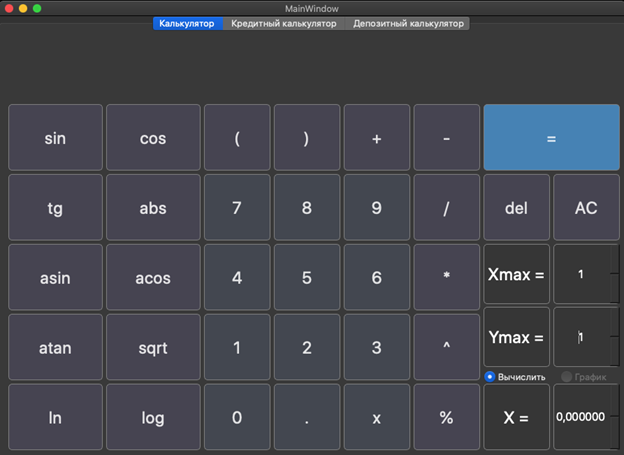
\includegraphics[bb=0 0 700 450]{media/image1.png}

\pagebreak[10]
\huge
\textbf{Основные функции}
\newline

\LARGE
Калькулятор поддерживает целые числа, запись вещественных чисел через точку и
в экспоненциальной форме, а так же следующие математические операции:
\newline
\textbf{Арифметические операции:}


\begin{itemize}
\item
  
  Сложение -- `a + b'
  
\item
  
  Вычитание -- `a -- b'
  
\item

  Умножение -- `a * b'

\item

  Деление -- `a / b'

\item

  Возведение в степень -- `a \^{} b'

\item

  Остаток от деления -- `a \% b'

\item

  Унарный минус -- `-a'

\end{itemize}


\textbf{Функции:}


\begin{itemize}
\item

  Синус -- `sin(a)'

\item

  Косинус -- `cos(a)'

\item

  Тангенс -- `tg(a)'

\item

  Модуль -- `abs(a)'

\item

  Арксинус -- `asin(a)'

\item

  Арккосинус -- `acos(a)'

\item

  Арктангенс -- `atan(a)'

\item

  Корень числа -- `sqrt(a)'

\item

  Натуральный логарифм -- `ln(a)'

\item

  Логарифм по основанию 10 -- `log(a)'

\end{itemize}
\pagebreak[10]
\huge
\textbf{Построение графика}
\newline

\LARGE
Наличие
во вводимом выражении переменной \textbf{`x'} позволит построить график
введённой функции.

Пользователю доступен выбор ввести конкретное значение \textbf{`x'} и
вычислить результат как обычное выражение или выбрать параметр
\textbf{``график''} и указать область определения и область значения
(\textbf{Xmax} и \textbf{Ymax}) на которых будет производиться расчёт.

График строится в отдельном открывающемся окне.
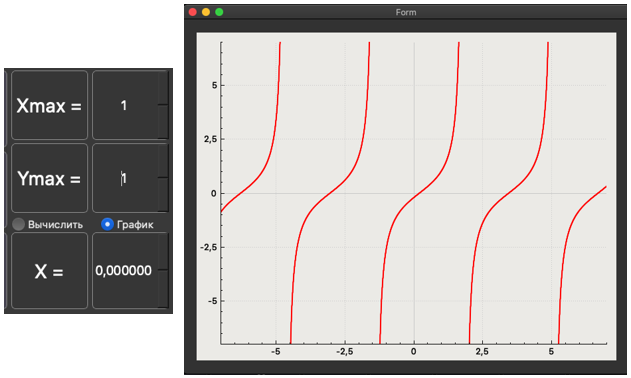
\includegraphics[bb=0 0 500 350]{media/image2.png}

\pagebreak[25]

\huge
\textbf{Кредитный калькулятор}
\newline

\LARGE
В кредитном калькуляторе пользователь вбивает сумму кредита. Выбирает
срок, на который берёт этот кредит. Указывает процентную ставку и
выбирает тип платежей, аннуитетные или дифференцированные.

На выходе пользователь получает:

\begin{itemize}
\item
  ежемесячный платёж;
\item
  переплату по кредиту;
\item
  общую выплату.
\end{itemize}

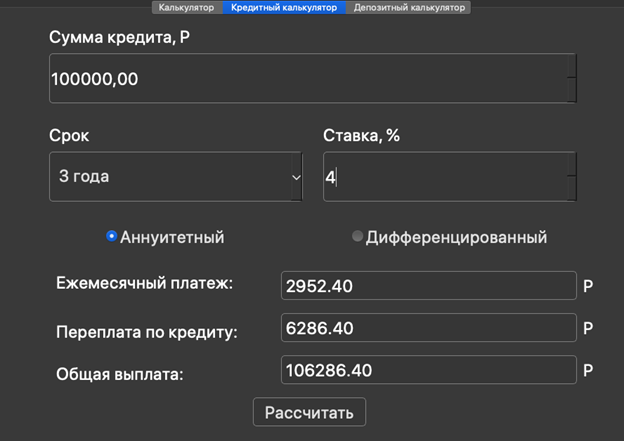
\includegraphics[bb=0 0 700 450]{media/image4.png}

\end{document}
